% Edited conversion of source pp. 41--42.
\ReportHeading
  {Моделювання крейзів у привершинних зонах тріщин між двома п’єзоелектричними матеріалами}
  {А.~Є. Шевельова, Р.~О. Щербак, Т.~В. Ходанен}
  {Дніпровський національний університет імені Олеся Гончара}
  {}

П’єзоелектричні матеріали характеризуються сильним зв’язком між електричними та механічними полями й широко використовуються у датчиках, виконавчих механізмах та системах точного керування. Водночас п’єзокераміка є механічно крихкою, тому в композитних елементах тріщини часто виникають уздовж меж поділу. Якщо компоненти з’єднані тонким полімерним клейовим шаром, руйнування цього шару може відбуватися через утворення крейзів --- локалізованих мікродефектів, заповнених орієнтованими фібрилами та порами.

Розглянуто біматеріал із двох напівнескінченних п’єзоелектричних областей $x_3>h/2$ та $x_3<-h/2$. Обидва матеріали належать до класу симетрії $6mm$, а їхні осі поляризації спрямовані вздовж $x_3$. Області з’єднані клейовим шаром товщиною $h$, який характеризується модулем зсуву $\mu$, коефіцієнтом Пуассона $\nu$ та границею текучості $\sigma_Y$.

На нескінченності задано рівномірні механічні навантаження й електричне зміщення
\[
 \sigma_{33}^{(m)}=\sigma,\qquad
 \sigma_{13}^{(m)}=\tau,\qquad
 D_3^{(m)}=d,\qquad m=1,2,
\]
де $m=1$ відповідає верхній, а $m=2$ --- нижній області. Оскільки навантаження не залежить від $x_2$, задачу розглянуто у площині $(x_1,x_3)$.

Тріщина $(a,b)$ може лежати на межі клейового шару з однією з матриць або всередині шару. Через нижчу жорсткість адгезиву руйнування починається з локалізованих зон передруйнування $[a_1,a]$ та $[b,b_1]$, які моделюють крейзи.

\begin{figure}[htbp]
\centering
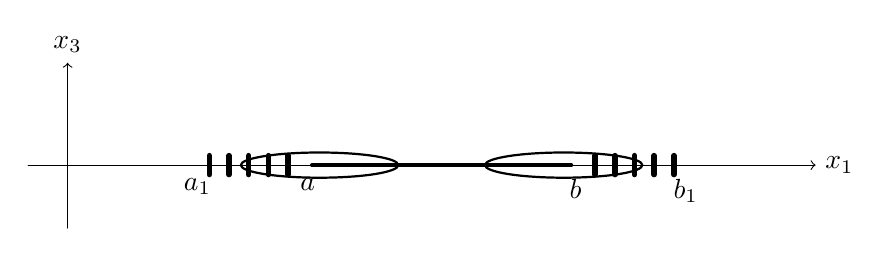
\begin{tikzpicture}[x=1.0cm,y=1.0cm,line cap=round,line join=round]
  \draw[->] (-0.5,0)--(9.5,0) node[right] {$x_1$};
  \draw[->] (0,-0.8)--(0,1.3) node[above] {$x_3$};
  \draw[very thick] (3.1,0)--(6.4,0);
  \draw[thick] (3.2,0) ellipse (1.0 and 0.16);
  \draw[thick] (6.3,0) ellipse (1.0 and 0.16);
  \foreach \x in {1.8,2.05,2.30,2.55,2.80} {\draw[line width=2pt] (\x,-0.12)--(\x,0.12);}
  \foreach \x in {6.70,6.95,7.20,7.45,7.70} {\draw[line width=2pt] (\x,-0.12)--(\x,0.12);}
  \node[below] at (1.65,-0.05) {$a_1$};
  \node[below] at (3.05,-0.05) {$a$};
  \node[below] at (6.45,-0.05) {$b$};
  \node[below] at (7.85,-0.05) {$b_1$};
\end{tikzpicture}
\caption{Крейзові зони на продовженні міжфазної тріщини.}
\end{figure}

Через малу довжину крейзів порівняно з довжиною тріщини напруження у фібрилах кожної зони вважаються сталими. Для лівої зони
\[
 \sigma_{zz}=\sigma',\qquad \tau_{xz}=\tau',\qquad \sigma_{xx}=0,
\]
а для правої
\[
 \sigma_{zz}=\sigma,\qquad \tau_{xz}=\tau,\qquad \sigma_{xx}=0.
\]
Для кожної зони прийнято умову текучості Мізеса; для правої зони її записано у формі
\begin{equation}
 f(\sigma,\tau,\sigma_1)
 =(\sigma-\sigma_1)^2+4\tau^2-\frac{4}{3}\sigma_T^2=0.
\end{equation}

Детально досліджено модель із двома фібрилами. Методом комплексних потенціалів побудовано подання електромеханічних полів на межі поділу матеріалів. Разом з умовою текучості це дало трансцендентні рівняння для визначення довжин зон передруйнування, напружень у цих зонах та розкриття тріщини. Підхід проілюстровано для конкретних комбінацій матеріалів і навантажень.

\textit{Роботу виконано за фінансової підтримки Національного фонду досліджень України, грант №~2025.07/0117.}
